%% ACL submission — Cultural contextualization reasoning
%% Compile: pdflatex paper.tex && bibtex paper && pdflatex paper.tex && pdflatex paper.tex

\documentclass[11pt]{article}
\usepackage[review]{acl}
\usepackage{times}
\usepackage{latexsym}
\usepackage[T1]{fontenc}
\usepackage[utf8]{inputenc}
\usepackage{microtype}
\usepackage{inconsolata}
\usepackage{graphicx}
\usepackage{booktabs}
\usepackage{multirow}
\usepackage{amsmath}
\usepackage{xcolor}
\usepackage{tikz}
\usetikzlibrary{positioning, arrows.meta}

\title{Cultural Contextualization Reasoning}

\author{Anonymous ACL Submission}

\begin{document}
\maketitle

%% ============================================================
\begin{abstract}
Large language models collapse cultural reasoning into a single dominant
chain-of-thought pathway, failing to reflect the plurality of cultural
perspectives present across human communities.
We address this limitation by constructing a \textbf{Cultural Knowledge
Graph} (CKG) whose structure mirrors the way cultural knowledge is
actually organized: rooted in the universal concept of \emph{Human} and
branching outward through increasingly fine-grained cultural
representations spanning domains, groups, practices, and specific
cultural cues.
As a first step toward this goal, we mine five publicly available cultural
commonsense datasets — CANDLE, ArabCulture, DIWALI, CultureBank, and
BLEnD — using a structured LLM-assisted extraction pipeline.
The resulting graph contains \textbf{7,542 nodes} and \textbf{8,639
directed edges} across five abstraction levels and eight culturally
grounded relation types, covering 279 cultural domains and over
500 distinct cultural groups drawn from more than 20 countries.
We describe the dataset selection rationale, graph schema design, and
extraction methodology, and present an analysis of the extracted graph's
coverage, connectivity, and relation diversity.
\end{abstract}

%% ============================================================
\section{Introduction}

Cultural reasoning is an inherently non-linear process.
Where conventional chain-of-thought prompting leads a language model
along a single inferential path, cultural understanding demands the
simultaneous navigation of multiple, often parallel, interpretive
frameworks shaped by religion, family, community, gender, economy, and
tradition.
A Muslim and a secular Westerner presented with the same scenario —
sharing a meal, greeting a stranger, negotiating a contract — will arrive
at different conclusions not because one is incorrect, but because each
draws on a distinct cultural knowledge pathway.

Contemporary LLMs are trained predominantly on English-dominant, Western
internet data.
When asked to reason about culturally situated scenarios, these models
default to the cultural majority, effectively silencing minority
perspectives \cite{myung2024blend,shi2024culturebank}.
The problem is not a lack of cultural knowledge per se — large models do
contain substantial cultural information — but a failure of
\emph{contextualization}: the capacity to activate, weight, and
articulate the appropriate cultural pathway for a given context.

We propose a framework for \textbf{cultural contextualization reasoning}
grounded in a hierarchical Cultural Knowledge Graph (CKG).
The graph encodes cultural knowledge along a continuum from the abstract
(\emph{Human}) to the concrete (\emph{specific cultural cue}), with
edges labeled by culturally informed relation types that replace the
reductive causal ``leads to'' with relations such as \emph{honors},
\emph{balances}, \emph{contextualizes}, and \emph{varies by}.
This structure supports multi-path reasoning: given a scenario, an expert
model may traverse several cultural pathways simultaneously, producing a
richer, more representative response.

This paper reports the first phase of this project: the construction of
the CKG via text mining of existing cultural commonsense datasets.
Subsequent phases will build on this graph to develop recursive agentic
reasoning frameworks, reinforcement learning-based pathway selection, and
retrieval-augmented generation for culturally contextualized response
generation.

%% ============================================================
\section{Datasets}
\label{sec:datasets}

We selected six datasets that collectively span a wide range of cultural
groups, geographical regions, and commonsense knowledge types.
Table~\ref{tab:datasets} summarizes their key properties.

\begin{table*}[t]
\centering
\small
\begin{tabular}{llllr}
\toprule
\textbf{Dataset} & \textbf{Reference} & \textbf{Coverage} & \textbf{Format} & \textbf{Size} \\
\midrule
CANDLE    & \citet{nguyen2023candle}   & 386 cultural groups, 60K clusters & Assertions (JSONL) & 1.1M \\
ArabCulture & \citet{sadallah2025arab} & 13 Arab countries                 & MCQ scenarios      & 3,482 \\
DIWALI    & \citet{sahoo2025diwali}    & 36 Indian states, 17 facets       & Concept descriptions & 8,817 \\
CultureBank & \citet{shi2024culturebank} & 730 cultural groups (TikTok/Reddit) & Behavioral norms & 23,000 \\
BLEnD     & \citet{myung2024blend}     & 16 countries, 13 languages        & QA pairs           & 52,600 \\
Ko-PIQA   & \citet{choi2025kopiqa}     & Korean cultural cues              & Physical QA        & 441 \\
\bottomrule
\end{tabular}
\caption{Datasets used for cultural knowledge graph construction.
Ko-PIQA was not yet publicly available at the time of this work.}
\label{tab:datasets}
\end{table*}

\paragraph{CANDLE} \cite{nguyen2023candle} is a large-scale cultural
commonsense knowledge base containing over 1.1 million assertions about
386 cultural groups extracted from web text.
Assertions cover six facets (food, clothing, traditions, rituals,
behaviors, norms) and are scored for frequency, distinctiveness, and
relevance.
CANDLE provides the broadest occupational and societal group coverage of
any dataset in our collection.

\paragraph{ArabCulture} \cite{sadallah2025arab} is a multiple-choice
commonsense reasoning dataset covering 13 Arab countries across the
MENA region.
Each instance presents a culturally situated scenario alongside distractor
options, requiring models to select the culturally appropriate response.
The dataset captures intra-Arab cultural variation — e.g., practices that
are common in Egypt but not in the UAE.

\paragraph{DIWALI} \cite{sahoo2025diwali} provides 8,817 culture-specific
concept descriptions spanning 36 Indian states and 17 cultural facets
including textiles, cuisine, dance, architecture, and festivals.
Its fine-grained regional breakdown makes it particularly valuable for
capturing sub-national cultural diversity within a single country.

\paragraph{CultureBank} \cite{shi2024culturebank} is derived from TikTok
and Reddit posts and encodes behavioral norms as structured tuples
(cultural group, context, goal, actor behavior, recipient behavior).
Its grounding in social media makes it especially sensitive to
contemporary and contested cultural practices.

\paragraph{BLEnD} \cite{myung2024blend} is a multilingual benchmark
covering everyday cultural knowledge across 16 countries and 13
languages.
Each question is posed in the local language alongside an English
translation, making BLEnD the most linguistically diverse dataset in our
collection.

\paragraph{Ko-PIQA} \cite{choi2025kopiqa} is a Korean physical
commonsense reasoning dataset with cultural annotations.
It was not yet publicly available at the time of this work and is
reserved for future phases of the project.

%% ============================================================
\section{Methodology}
\label{sec:methodology}

\subsection{Graph Schema}
\label{sec:schema}

We design the Cultural Knowledge Graph around a five-level abstraction
hierarchy that moves from the universal to the culturally specific:

\begin{enumerate}
    \item[\textbf{L0}] \textbf{Human} — the universal root node,
    representing all humanity as the origin point of cultural knowledge.
    \item[\textbf{L1}] \textbf{Cultural Domain} — high-level thematic
    categories such as \emph{religion}, \emph{family}, \emph{food},
    \emph{economy}, \emph{tradition}, \emph{language}, \emph{gender},
    \emph{community}, \emph{art}, \emph{health}, \emph{education},
    \emph{politics}, \emph{nature}, and \emph{identity}.
    \item[\textbf{L2}] \textbf{Cultural Group} — a named community or
    identity (e.g., \emph{Algerian}, \emph{American}, \emph{Andhra
    Pradesh}, \emph{teacher}).
    \item[\textbf{L3}] \textbf{Cultural Practice / Belief / Norm} — a
    behavioral or normative pattern associated with a group
    (e.g., \emph{fasting during Ramadan},
    \emph{removing shoes indoors},
    \emph{arranged marriage practice}).
    \item[\textbf{L4}] \textbf{Specific Instance / Cue} — a concrete
    action, object, or artifact
    (e.g., \emph{not eating from sunrise to sunset},
    \emph{15--30\% tip percentage},
    \emph{Pochampally Ikat textile}).
\end{enumerate}

\noindent Figure~\ref{fig:schema} illustrates this hierarchy with
an example pathway rooted in the \emph{economy} domain.

\begin{figure}[h]
\centering
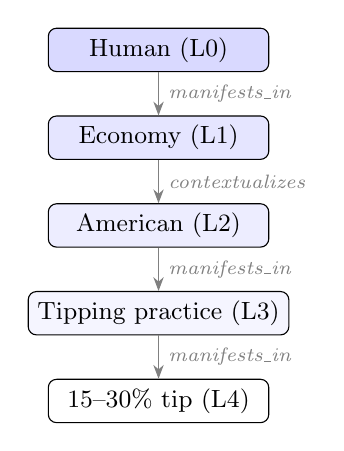
\begin{tikzpicture}[
    node distance=0.55cm and 1.2cm,
    every node/.style={font=\small, align=center},
    box/.style={draw, rounded corners=3pt, fill=gray!10,
                minimum width=2.8cm, minimum height=0.55cm},
    arr/.style={-{Stealth[length=5pt]}, gray}
]
\node[box, fill=blue!15] (l0) {Human (L0)};
\node[box, fill=blue!10, below=of l0] (l1) {Economy (L1)};
\node[box, fill=blue!7, below=of l1] (l2) {American (L2)};
\node[box, fill=blue!4, below=of l2] (l3) {Tipping practice (L3)};
\node[box, fill=white, below=of l3] (l4) {15--30\% tip (L4)};
\draw[arr] (l0) -- node[right, font=\scriptsize]{\emph{manifests\_in}} (l1);
\draw[arr] (l1) -- node[right, font=\scriptsize]{\emph{contextualizes}} (l2);
\draw[arr] (l2) -- node[right, font=\scriptsize]{\emph{manifests\_in}} (l3);
\draw[arr] (l3) -- node[right, font=\scriptsize]{\emph{manifests\_in}} (l4);
\end{tikzpicture}
\caption{Example cultural reasoning pathway from the abstract root
(\emph{Human}) to a concrete cultural cue (\emph{15--30\% tip
percentage}).}
\label{fig:schema}
\end{figure}

\paragraph{Edge relation types.}
A central design decision is the replacement of reductive causal edges
(\emph{leads to}) with eight culturally informed relation types that
better reflect the relational and contextual nature of cultural knowledge
\cite{tonga2026llms}:

\begin{itemize}
    \item \textbf{manifests\_in} — an abstract concept is expressed
    through a more concrete one.
    \item \textbf{contextualizes} — a group or domain provides the
    interpretive frame for a practice.
    \item \textbf{influences} — one element shapes another without
    determining it.
    \item \textbf{varies\_by} — a practice differs across groups or
    contexts.
    \item \textbf{originates\_from} — a practice or norm derives from a
    belief or tradition.
    \item \textbf{honors} — a practice expresses respect for a cultural
    value.
    \item \textbf{balances} — competing cultural imperatives are held in
    tension.
    \item \textbf{restricts} — a cultural norm limits a behavior.
\end{itemize}

\subsection{LLM-Assisted Extraction Pipeline}
\label{sec:pipeline}

Each dataset entry is processed by a structured extraction pipeline
(Figure~\ref{fig:pipeline}) that produces a set of typed nodes and
labeled edges.

\begin{figure}[h]
\centering
\small
\begin{tabular}{l}
\toprule
\textbf{Input:} dataset entry (text, cultural group, metadata) \\
\midrule
1.\ Prompt Claude (\texttt{claude-haiku-4-5}) with \\
\quad cached system prompt defining schema \\
2.\ Parse JSON response: nodes $+$ edges \\
3.\ Normalize labels (lowercase, domain coercion) \\
4.\ Deduplicate nodes (increment frequency) \\
5.\ Deduplicate edges (increment weight) \\
6.\ Anchor L1 nodes to Human root \\
\midrule
\textbf{Output:} typed node $+$ labeled edge lists \\
\bottomrule
\end{tabular}
\caption{Extraction pipeline for a single dataset entry.}
\label{fig:pipeline}
\end{figure}

\paragraph{Prompt design.}
The system prompt is sent once per session with prompt caching enabled
\cite{anthropic2024caching}, substantially reducing API cost across the
2,500-entry run.
It instructs the model to extract 2–8 nodes per entry classified by
level (L0–L4), cultural group, and domain, and to connect them using only
the eight permitted relation types.
The model is explicitly instructed that edge labels must match node labels
exactly and that labels must be short (1–5 words), lowercase, and in
English.

\paragraph{Post-processing.}
Extracted nodes are normalized to lowercase and validated against the
domain taxonomy.
Nodes with unrecognized domains are assigned the \emph{unknown} class.
Edges whose endpoints are not present in the node set are discarded.
All Level~1 domain nodes are automatically connected to the Human root
via \emph{manifests\_in} edges to ensure a fully anchored hierarchy.

%% ============================================================
\section{Results and Analysis}
\label{sec:results}

We ran the pipeline on 500 entries from each of the five available
datasets (2,500 entries total), using the
\texttt{claude-haiku-4-5-20251001} model.
Table~\ref{tab:results} reports key graph statistics.

\begin{table}[h]
\centering
\small
\begin{tabular}{lr}
\toprule
\textbf{Metric} & \textbf{Value} \\
\midrule
Total nodes             & 7,542 \\
Total edges             & 8,639 \\
Level 0 (Human root)    & 1 \\
Level 1 (Domains)       & 279 \\
Level 2 (Groups)        & 552 \\
Level 3 (Practices)     & 3,312 \\
Level 4 (Instances)     & 3,398 \\
\midrule
Distinct cultural groups & 552 \\
Countries / regions covered & 20+ \\
Largest connected component & 7,183 (95.2\%) \\
Avg.\ out-degree        & 1.12 \\
\bottomrule
\end{tabular}
\caption{Cultural Knowledge Graph statistics after extraction
from 2,500 dataset entries across five datasets.}
\label{tab:results}
\end{table}

\paragraph{Node contribution by dataset.}
CultureBank contributed the most nodes (2,001), followed by DIWALI
(1,642), CANDLE (1,423), ArabCulture (1,273), and BLEnD (1,202).
The variation reflects both dataset size and the density of extractable
cultural knowledge per entry.

\paragraph{Edge diversity.}
\emph{Manifests\_in} accounts for 70.3\% of edges, consistent with its
role as the primary hierarchical connector.
The remaining 29.7\% of edges encode richer relational semantics:
\emph{contextualizes} (14.2\%), \emph{influences} (5.4\%),
\emph{varies\_by} (4.0\%), \emph{originates\_from} (2.9\%),
\emph{honors} (1.6\%), \emph{balances} (1.1\%), and
\emph{restricts} (0.4\%).

\paragraph{Domain coverage.}
The most populated domains are \emph{art} (1,596 nodes),
\emph{tradition} (1,026), \emph{economy} (1,001), \emph{food} (893),
\emph{education} (573), and \emph{family} (538).
\emph{Religion}, \emph{gender}, and \emph{politics} are less populated,
pointing to gaps in the underlying datasets that future work should
address.

\paragraph{Cultural group coverage.}
The top groups include Algerian (1,504 nodes), general (1,078), American
(791), Egyptian (365), and a rich set of Indian regional groups (Andhra
Pradesh, Assam, Chhattisgarh, Bihar).
CANDLE's treatment of occupational groups (teacher, nurse, attorney) as
cultural communities introduces an interesting dimension: professional
culture as a form of cultural identity.

\paragraph{Graph connectivity.}
95.2\% of nodes belong to the single largest connected component,
confirming that the anchoring strategy (connecting all L1 domain nodes to
the Human root) effectively unifies the graph.
The 220 smaller components correspond to culturally specific subgraphs
that share no direct pathway with the main hierarchy — a potential target
for future cross-cultural bridge edge construction.

%% ============================================================
\section{Related Work}
\label{sec:related}

\subsection{Graph-Based Cultural Knowledge}

\citet{tonga2026llms} demonstrate that LLMs can serve as cultural
archives by extracting cultural commonsense knowledge graphs from
pretraining data.
Their work focuses on extraction fidelity; our contribution extends this
by imposing a principled five-level abstraction hierarchy and a richer
relational vocabulary designed to support multi-path reasoning rather than
single-path retrieval.

\subsection{Cultural NLP Benchmarks}

A growing body of work has developed benchmarks to evaluate cultural
sensitivity in LLMs
\cite{nguyen2023candle, sadallah2025arab, sahoo2025diwali,
shi2024culturebank, myung2024blend, choi2025kopiqa}.
These datasets have primarily been used for model evaluation.
We repurpose them as a mining corpus for knowledge graph construction,
treating their cultural instances as raw material for structured
representation rather than as test cases.

%% ============================================================
\section{Conclusion and Next Steps}
\label{sec:conclusion}

We have presented the first component of a cultural contextualization
reasoning framework: a Cultural Knowledge Graph mined from five datasets
using an LLM-assisted extraction pipeline.
The resulting graph — 7,542 nodes, 8,639 edges, 95\% connected —
provides a structured foundation for multi-path cultural reasoning.

Immediate next steps include:
\begin{itemize}
    \item \textbf{Task 2:} Provide the CKG schema to LLMs and instruct
    them to associate raw cultural text with graph columns, collecting
    diverse cultural interpretation outcomes to identify gaps and biases.
    \item \textbf{Task 3:} Survey philosophical and anthropological
    frameworks (e.g., work by Prof.\ Igor in Waterloo University) to
    validate and extend the abstraction hierarchy.
    \item \textbf{Task 4:} Design a recursive agentic framework that
    traverses the CKG to produce culturally diverse, multi-path
    responses to arbitrary scenarios.
\end{itemize}

%% ============================================================
\bibliography{references}

\appendix
\section{Graph Schema Reference}

\begin{table}[h]
\centering
\small
\begin{tabular}{lll}
\toprule
\textbf{Level} & \textbf{Name} & \textbf{Examples} \\
\midrule
L0 & Human & human \\
L1 & Domain & religion, food, family \\
L2 & Group  & algerian, american, bihar \\
L3 & Practice & fasting, tipping, shoe removal \\
L4 & Instance & 15--30\% tip, not eating pork \\
\bottomrule
\end{tabular}
\caption{CKG node level taxonomy.}
\end{table}

\begin{table}[h]
\centering
\small
\begin{tabular}{ll}
\toprule
\textbf{Relation} & \textbf{Semantics} \\
\midrule
manifests\_in    & abstract expressed as concrete \\
contextualizes   & provides interpretive frame \\
influences       & shapes without determining \\
varies\_by       & differs across groups/contexts \\
originates\_from & derived from belief/tradition \\
honors           & expresses respect for value \\
balances         & holds competing values in tension \\
restricts        & limits a behavior \\
\bottomrule
\end{tabular}
\caption{CKG edge relation type taxonomy.}
\end{table}

\end{document}
